% -/\/\/\/\/\/\/\/\/\/\/\/\/\/\/\/\/\/\/\/\/\/\/\/\/\/\/\/\/\/\/\/\/\/\/\/\/\/\/\/\/\/\/\/\/\/\/\/\/\/\/\/\/\/\/\/\/\/\/\/\/\/\/\/\/\/\/\/\/\/\/\/\/\/\/\/\/\/\/\/\/\-
%  -X-X-X-X-X-X-X-X-X-X-X-X-X-X-X-X-X-X-X-X-X-X-X-X-X-X-X-X-X-X-X-X-X-X-X-X-X-X-X-X-X-X-X-X-X-X-
% -\/\/\/\/\/\/\/\/\/\/\/\/\/\/\/\/\/\/\/\/\/\/\/\/\/\/\/\/\/\/\/\/\/\/\/\/\/\/\/\/\/\/\/\/\/\/\/\/\/\/\/\/\/\/\/\/\/\/\/\/\/\/\/\/\/\/\/\/\/\/\/\/\/\/\/\/\/\/\/\/\/-
\documentclass[10pt]{article}
\usepackage{geometry} 
\usepackage{indentfirst}
\usepackage{hyperref}
\usepackage{color}
\usepackage{comment}
\usepackage[pdftex]{graphicx}  
\usepackage{caption}
\usepackage{natbib}
\usepackage{mathtools}
\usepackage{units}
\usepackage{booktabs}
\usepackage{authblk}
\renewcommand{\baselinestretch}{1.5}
\geometry{a4paper} 
\bibliographystyle{apalike}
\graphicspath{{../graphs/}} % Location of the graphics files

%nouvelle commande pour les commentaires
\newcommand{\sme}[1]{\textcolor{red}{\bf #1}}
\newcommand{\yang}[1]{\textcolor{blue}{\bf #1}}
\newcommand{\beginsupplement}{%
        \setcounter{table}{0}
        \renewcommand{\thetable}{S\arabic{table}}%
        \setcounter{figure}{0}
        \renewcommand{\thefigure}{S\arabic{figure}}%
     }


%\usepackage[utf8]{inputenc} => pour les accents

% -/\/\/\/\/\/\/\/\/\/\/\/\/\/\/\/\
%\chapter
%\section
%\subsection
%\subsubsection
%\subsubsection
%\paragraph
%\subparagraph
% -\/\/\/\/\/\/\/\/\/\/\/\/\/\/\/\/

%----------------------------------------
%AUTHORS
%----------------------------------------

\title{Heterosis and genetic load in an ExPVP partial diallel cross} 

\author[1]{Jinliang Yang\thanks{jolyang@ucdavis.edu}}
\author[1,2,3]{Sofiane Mezmouk\thanks{smezmouk@ucdavis.edu}}
\author[4]{Rita H. Mumm\thanks{ritamumm@illinois.edu}}
\author[1,2]{Jeffrey Ross-Ibarra\thanks{rossibarra@ucdavis.edu}}
\affil[1]{Department of Plant Sciences, University of California, Davis, CA 95616, USA}
\affil[2]{Center for Population Biology and Genome Center, University of California Davis}
\affil[3]{Current address: KWS SAAT AG, Grimsehlstr. 31, 37555 Einbeck, Germany}
\affil[4]{Department of Crop Sciences, University of Illinois at Urbana-Champaign, Urbana, IL 61801, USA}

\date{}


%-----------------------------------------------------------------------------------------------------------------
%-----------------------------------------------------------------------------------------------------------------
% BEGIN DOCUMENT
%-----------------------------------------------------------------------------------------------------------------
%-----------------------------------------------------------------------------------------------------------------
\begin{document}

\maketitle
%----------------------------------------
% ABSTRACT
%----------------------------------------
\newpage

\section*{Abstract}

%The story is: I have a partial diallel cross with both phenotypic and genotypic data and I observe over dominance at haplotypic level but at the SNP level; everything is explained by dominance. 

Genomic selection (GS) has gained popularity recently as the availability of genome-wide markers has increased. Current methods for GS weigh all the available SNPs equally in model training, without considering their functional differences. Genetic variations detected at evolutionary conserved sites tend to be deleterious and, thus, may be more informative for GS. To utilize this kind of information as a prior into the GS model, we proposed a method to put more weight on evolutionarily constrained sites. As a proof-of-concept, a half diallel population based on 12 diverse inbred lines was used, from which seven phenotypic traits were collected. Some of these traits show high levels of heterosis. After sequencing the 12 founder lines, about 14 million SNPs were discovered and the SNPs were used to identify 502,913 haplotype blocks shared through identity by descent (IBD). A five fold cross-validation experiment was conducted using the summary statistics of the SNP conservation scores, which were computed by evaluating sequences similarity of multiple divergent species, in the IBD blocks as explanatory variables. The results show that the prediction accuracies are significantly better than shuffled data with randomly assigned conservation scores. This study demonstrates the importance of incorporating evolutionary information in GS and its potential use in plant breeding.




%----------------------------------------
% INTRODUCTION
%----------------------------------------
\newpage
\section*{Introduction}
%----------------------------------------

%\textbf{Prediction approach for deleterious alleles} 

\textbf{Why we care about deleterious variants. Discuss results of Mezmouk 2014. We are extending this in three ways}  
\begin{itemize}
  \item all deleterious SNPs not just coding
  \item genome-wide not just reduced representation
  \item using GS to test whether they improve prediction
\end{itemize}


%\textbf{Heterosis was observed long time ago. many theories were proposed to explain it.}

The phenomenon of heterosis has been observed for many species across taxa, from yeast \citep{Shapira2014} to vertebrates \citep{Gama2013}. Although heterosis has been broadly applied for food production and has been extensively studied by many researchers, the underlying mechanism controlling for it remains elusive. Recent studies indicated that the complementation of the deleterious alleles, which fit the classical dominance genetic model, may play an important role in determining heterosis \citep{Charlesworth2009}. Deleterious alleles were arisen from new mutations during meiosis. In maize, about 90 new mutations were generated per meiosis \citep{Clark2005}, majority of which were deemed to be deleterious according to empirical estimates \citep{Joseph2004}. In a natural outcross population, the negative effects on fitness of these deleterious alleles make them subject to be selected against. Therefore, deleterious alleles were mainly maintained in a low frequency \citep{Eyre-Walker2007}. 

%\textbf{Many new mutations, most deleterious}

%~90 mutations per meiosis (Clark et al. 2005 MBE, Jiao et al. 2012 Nature Genetics), maize HapMap2 new mutations of large effect (Hufford et al 2012 Nature Genetics, Soletzki 2011 MBE).
%Purifying selection retards recovery of diversity in genic regions.

%pesudo-overdominance model
In maize, the total number of mildly deleterious mutations is substantial because of the exponential growth of population size after domestication. The modern breeding probably aims to remove these deleterious mutations and pyramiding beneficial alleles for agronomical important traits. In practice, the relatively homogeneous maize germplasm pool was artificially divided into different heterotic groups \citep{Heerwaarden2012}. It enabled the improvement of germplasm pools to be conducted in a parallel fashion. By doing this, the maize yield has been steadily improved since the early 20th century \yang{citation}. However, the removing of deleterious mutations in low recombination regions or in tightly linked regions is less effective. Studies indicated that residual heterozygosity correlates negatively with recombination \citep{Gore2009, McMullen2009} and the low recombination is effective over long period of time \citep{Haddrill2007}. As a consequence, the deleterious alleles would be accumulated in the pericentromeric region and the vigorous performance could only be realized by combining two sets of non-deleterious or beneficial alleles in repulsion state, thus lead to pesudo-overdominance. Recent QTL study identified loci controlling for heterosis are enriched in centromeric regions \citep{Lariepe2012}, which may support this pesudo-overdominance hypothesis.

To study the relationship between deleterious variants, especially those with minor effect or rare in the population, and their contribution to heterosis, a diallel population was employed \citep{}. This diallel population enabled us to invistigate the different modes of inheritance of the deleterious variant in a hybrid population with super dense SNP markers; while only relative little sequencing efforts need to be conducted on founder lines. Our previous study observed that an excess of deleterious SNPs were enriched in GWAS set \citep{Mezmouk2014}. In that study, deleterious variants were defined as nonsynonymous mutations. Clearly, deleterious varinats are not limitted to coding regions. Here, we expanded the characterization of deleterious variants to genome wide by using genomic evolutionary rate profiling (GERP) \citep{Cooper2005}. GERP scores were obtained by computing the regected substitutions subtracted by the neutral rate after multiple sequence alignment of a set of related species \citep{Davydov2010}. \yang{Sofina's GWAS results.}. Because most of the deleterious alleles are rare, their effects are difficult to be detected by traditional GWAS approach. To overcome it, a genomic selection approach was conceived, which enable us to estimate the combined effects of all the possible deleterious variants simuteously. As the results, genomic selection with GERP score incorporated in the prediction model show better performance than circular shuffled data for some phentoypic traits. This study demonstrates the importance of incorporating evolutionary information in genomic selection and its potential use in plant breeding.
   


%----------------------------------------
% RESULTS
%----------------------------------------
\section*{Results}
%----------------------------------------

\begin{itemize}
  \item Genetic values, heritability, heterosis and combining ability 
  \item SNP calls and annotation; distribution of deleterious mutations along the genome 
  \item correlation between complementation at deleterious SNPs with heterosis and SCA for the different 
  \item IBD region size and general statistics 
  \item IBD correlation with heterosis and SCA
  \item GWAS results at an SNP level and then comparison with haplotypic results 
  \item Analyses of the significant haplotypic bloc to see if there is any pattern
\end{itemize}

\subsection*{Genetic values, heritability, heterosis and combining ability of a partial diallel population}

A half diallel population was created using 12 maize inbred lines. Two of them are important public inbreds, B73 and Mo17. And the other ten of them are (LH1, LH123HT, LH82, PH207, 4676A, PHG39, PHG47, PHG84, PHJ40, PHZ51) are proprietary inbreds that have expired from Plant Variety Protection (PVP) and represent the lineage of key heterotic germplasm pools used in present-day commercial corn hybrids. This diallel facilitated the creation of F1 hybrids that are adapted to the U.S., fairly elite in performance, and commercially relevant. The set is diverse enough to facilitate a broad sweep of the heterotic sub-groups that comprise U.S. commercial germplasm.


\subsection*{IBD region size and general statistics}

Identity by descent was esimated with fasibd.
Average size 44,980 bp (36 to 10,320,000 bp)
Figure 1: ~\ref{fig:mafmiss}.


Figure S1: ~\ref{fig:maf2}

\subsection*{GERP, SIFTMAPP and general statistics}

%GERP statistics
Introduce GERP SNP and GERP elements. For each position of the multiple alignment, the conservation score is computed in rejected substitution by subtracting the estimated evolutionary rate from the neutral rate (citation).
224,087 GERP elements were identified in B73v2. 
29,869,451 bps (1.4\% of the maize genome).


Figure S2. distribution of GERP, GERP vs. MAF.



Figure S3. GERP in gene, exon and intron.


\subsection*{Evolutionary conservation information improved prediction accuracies}

Figure S4. GERP in IBD design with additive and dominance model.

Some prior knowledge have not been used for model training. 
SNPs with high GERP score were considered as evolutionary conserved. The mutation at these sites tend to be deleterious. However, because SNPs with high GERP score are negatively correlated with the MAF (Figure and citation), they become less useful due to statistical limitation (citation). To capture the information carried by these potentially deleterious sites, we conducted the genomic-enabled prediction with the SNP's GERP score. 

The population in this study is relative small with only 66 individuals. The 20k conserved SNPs are highly colinear with others. To solve this problem, we use the haplotype-based approach for model training, where the haplotype was coded with the SNP conservation score as the explainatory variables. 

With a 5-fold cross-validation approach, the prediction accuracies of the real data and cicularly shuffled data were compared. To rule out the prossibility that genic SNPs are more conserved than intergenic ones. We elected the SNPs in genic regions and did the circular shuffling to random assign GERP scores the the same set of the selected SNPs.

As the results, for traits \emph{per se}, model prediction accuracies were significantly improved for ASI, DTS and PHT when incorporating GERP score information under the additive model. Prediction accuracies were significantly improved for ASI, DTP, GY and TW under the dominant model. In general, the average prediction rates are higher using the additive model (\emph{r} = 0.8) than the dominant model (\emph{r} = 0.7). For heterosis, incorporation of GERP scores only improved grain yield prediction and only under a dominant model.  


%----------------------------------------
% DISCUSSION
%----------------------------------------
\section*{Discussion}
%----------------------------------------


\begin{itemize}
  \item how do results match with heritability and heterosis?
  \item do we support deleterious model of Mezmouk et al.?
\end{itemize}

In this study, more than 500,000 deleterious SNPs were identified in elite maize lines including in noncoding regions of the genome. Majority of them were maintained in a low frequency, which consistent with the previous observation \yang{Eli PNAS, 2015} and indicate the deleteriousness of the variants in the conserved sites. A genomic selection pipeline was developed, which utilized evolutionary conservation information in the model.
Cross-validation results suggested prediction accuracies for some traits could be significantly improved by incorporating GERP scores. 



%----------------------------------------
% MATERIAL & METHODS
%----------------------------------------
\section*{Materials and methods}
%----------------------------------------

\subsection*{Plant material and phenotypic data}
%-------------------
Twelve maize inbred lines were selected and crossed in a partial diallel fashion without considering reciprocal effects \sme{(CITE)}. Ten of these inbreds (LH1, LH123HT, LH82, PH207, 4676A, PHG39, PHG47, PHG84, PHJ40, PHZ51) are proprietary inbreds that have expired from Plant Variety Protection (PVP) and represent the lineage of key heterotic germplasm pools used in present-day commercial corn hybrids, and two are predominant public inbreds B73 and Mo17.  \\

The experimental design includes the 66 F1 hybrids, the 12 inbred parents, and 2 current commercial check hybrids grown in an incomplete block design with 3 replications; hybrids and inbreds were grouped separately. The test was grown at Urbana, IL in 2009, 2010, and 2011.  Plots consisted of 4 rows, with all observations taken from the inside 2 rows to minimize effects of shading and maturity differences from adjacent plots. Both inbred lines and the 66 resulting hybrids were field evaluated. Phenotypic data was collected for plant height (PHT, in cm), ear height (EHT, in cm), days to 50\% silking (DTS), days to 50\% pollen shed (DTP), anthesis-silking interval (ASI, in days), grain yield adjusted to 15.5\% moisture (adj GY, in bu/A), and test weight (TWT, in pounds) \sme{(CITE)}.% Question for RHM: Should we cite a paper for the phenotypic data? 

\subsection*{Analyses}
%-------------------

\subsubsection*{Inbred line sequencing and SNP callings}

% wet lab
DNA from the twelve inbred lines was CTAB extracted \citep{Doyle1987} and Covaris sheared for Illumina library preparation. The DNA libraries were then sequenced to an average coverage of 10X \sme{(say where the sequencing was done?)}.

%Read mapping
Raw paired reads (reverse and forward for each sequence), were trimmed for adapter contamination with Scythe package (\url{https://github.com/vsbuffalo/scythe}) which calculate the probability of having a contamination given the adapter sequence, the number of mismatches and sequence quality. The reads were then trimmed for quality and sequence length ($\geq 20$ nucleotides) with Sickle package (\url{https://github.com/najoshi/sickle}) .

Read pairs, kept after filtering,  were mapped to the maize B73 reference genome (AGPv2) with bwa-mem \citep{Li2009B}. Reads, with mapping quality (MAPQ) higher than 10 and with a best alignment score higher than the second best one, were kept for further analyses.

%SNP calling
Single nucleotide polymorphisms (SNPs) were called with mpileup from samtools utilities \citep{Li2009}. To deal with paralogy, which is a major problem in maize sequence mapping \citep{Chia2012}, all SNPs were filtered to a) be heterozygote in less than 3 inbred lines, b) have a mean minor allele depth over all genomes of at least 4, c) have a mean depth over all individuals lower than 30 and d) have missing/heterozygote alleles in less than 6 inbred lines (allelic information for at least 15 hybrids in the partial diallel design). 

%SNP results after filtering
After filtering 13,782,809 are kept for further comparisons, including 1,909,416 genic SNPs and 361,280 in protein coding regions). \\
We estimated the allelic error rate by first comparing our genotype calls to those of 41,292 overlapping SNPs on the maize SNP50 bead chip \citep{Heerwaarden2012};  we then compared our SNP alleles for B73 and Mo17 with the 10,426,715 SNP previously identified in HapMap2 \citep{Chia2012}; finally, we compared our SNPs to 180,313 overlapping SNPs identified through Genotyping by sequencing \citep{Romay2013}. The comparisons showed 99.12\% allele similarity with shared SNPs previously identified. 


\subsubsection*{Haplotype identification and SNP annotation}

%IBD
All missing alleles were then imputed with BEAGLE package \citep{Browning2009} and identity by descent regions (IBD) between the 12 inbred lines were identified with BEAGLE's fastIBD method \citep{Browning2011}. The pairwise IBD region starts and ends were used to delimit haplotipic blocs where several inbred lines shared a homogenous haplotypes.%I need to clarify this last sentence.

%SIFT and MAPP
The SNPs were annotated as synonymous and non-synonymous with the software polydNdS from the analysis package of libsequence  \citep{Thornton2003} using the first transcript of each gene in B73 5b filtered gene set. Deleterious effects of amino acid changes were then predicted with both SIFT \citep{Ng2003, Ng2006} and MAPP \citep{Stone2005} software packages as described by \citep{Mezmouk2014}.

%GERP
Genomic evolutionary rate profiling (GERP) \sme{CITE}, which estimates the evolutionary constraint by quantifying substitution deficits after multiple genome alignments, was obtained from \yang{cite eli2015} for AGPv2. 



\subsubsection*{Phenotypic data analyses}

Best Linear Unbiased Estimation (BLUE) of the genetic effects were calculated with ASReml-R \sme{(CITE)} following the linear model \yang{check the following mixed linear model?}: 
%
\[y_{ijkl} = \mu + \varsigma_{i} + \delta_{ij} + \beta_{jk} + \alpha_{l} +  \varsigma_{i} \cdot \alpha_{l} + \varepsilon\]
%
where 
$y_{ijkl}$ is the phenotypic value of the $l^{th}$ genotype evaluated in the $k^{th}$ block of the $j^{th}$ replicate within the $i^{th}$ environment; 
$\mu$, the overall mean; 
$\varsigma_{i}$, the fixed effect of the $i^{th}$ environment;
$\delta_{ij}$, the fixed effect of the $j^{th}$ replicate nested in the $i^{th}$ environment; 
$\beta_{jk}$, the random effect of the $k^{th}$ block nested in the $j^{th}$ block; 
$\alpha_{l}$, the the fixed genetic effect  of the $l^{th}$ individual; 
$\varsigma_{i} \cdot \alpha_{l}$, the interaction effect of the $l^{th}$ individual with the $i^{th}$ environment; 
$\varepsilon$, the model residuals.

All fixed effects, including the genotype onces, were significant (Wald test p-value<0.05) for all traits except ASI for which the effect of the replicates within environments were not significant.

Heterosi for each hybrid was then estimated by both best- and mid-parent heterosis ($BPH$ and $MPH$, respectively):
%
\[ MPH_{ij}=\hat{G_{ij}}-\frac{1}{2}(\hat{G_{i}}+\hat{G_{j}}) \]
\[ BPH_{min,ij}=\hat{G_{ij}}-min(\hat{G_{i}} ,\hat{G_{j}}) \] 
\[ BPH_{max,ij}=\hat{G_{ij}}-max(\hat{G_{i}} ,\hat{G_{j}}) \]
%
where $\hat{G_{ij}}$, $\hat{G_{i}}$ and $\hat{G_{j}}$ are the genetic values of the hybrid and its two parents $i$ and $j$. $BPH_{min}$ was used instead of $BPH_{max}$ for days to anthesis.\\

Finally, general and specific combining ability (GCA ans SCA) respectively were estimated following \citet{Falconer1996}.

\subsubsection*{Association mapping}
SNP association with heterosis (BPH and MPH) was tested assuming dominance/recessivity of the reference allele or assuming overdominance where only the heterozygote alleles are expected to be significant. For each SNP, root mean square error were used to select the best fitting model. 
Haplotype association with heterosis were tested comparing the heterozygote alleles to all homozygote ones all confounded. 


\subsubsection*{Genomic-enabled prediction with GERP score}

A haplotype based genomic selection (GS) strategy was conceived by using the IBD blocks as the explanatory variables containing conservation information. The reference genome sites with GERP score />0 were considered as conserved sites and genomic variations at these sites were deemed as deleterious. To incoporate the conservation information into IBD blocks, SNPs falling into a given IBD block were added up using their GERP scores as the conservation estimates of the IBD block. This estimation was calculated using a python script gerpIBD (\url{https://github.com/RILAB/pvpDiallel}) with additive and dominant models. Under the additive model, 2 x GERP score was assigned to the homozygous loci with non-reference SNP calls; 1 x GERP score was assigned to the heterozygous loci; and 0 was assigned to the homozygous loci with reference SNP calls. Under the dominant model, 1 x GERP score was assigned to both the homzygous loci with non-reference SNP calls and heterozygous loci; 0 was assigned to homozygous loci with reference SNP calls.



seven phenotypic traits were trained with the conservation statistics in IBD block as genotype.
A Bayesian-based approach, BayesC \sme{CITE}, was employed for the GS experiments. To conduct predict, the diallel population was randomly divided into training and validation sets for 10 times according to a 5-fold cross-validation method. First, the BayesC model was trained independently on each of the training set. Second, the prediction accuracy was obtained by comparing the predicted and observed phenotypes on the conresponding validation set. 


In addition, the GERP scores were circularly shuffled. The cross-validation experiments using the circularly shuffled data were conducted on the same training and validation sets.  


%----------------------------------------
% REFERENCES
%----------------------------------------
\clearpage
\bibliography{Diallel}


%----------------------------------------
% FIGURES
%----------------------------------------
\pagebreak
\section*{Figures and Tables}

\begin{center}\vspace{1cm}
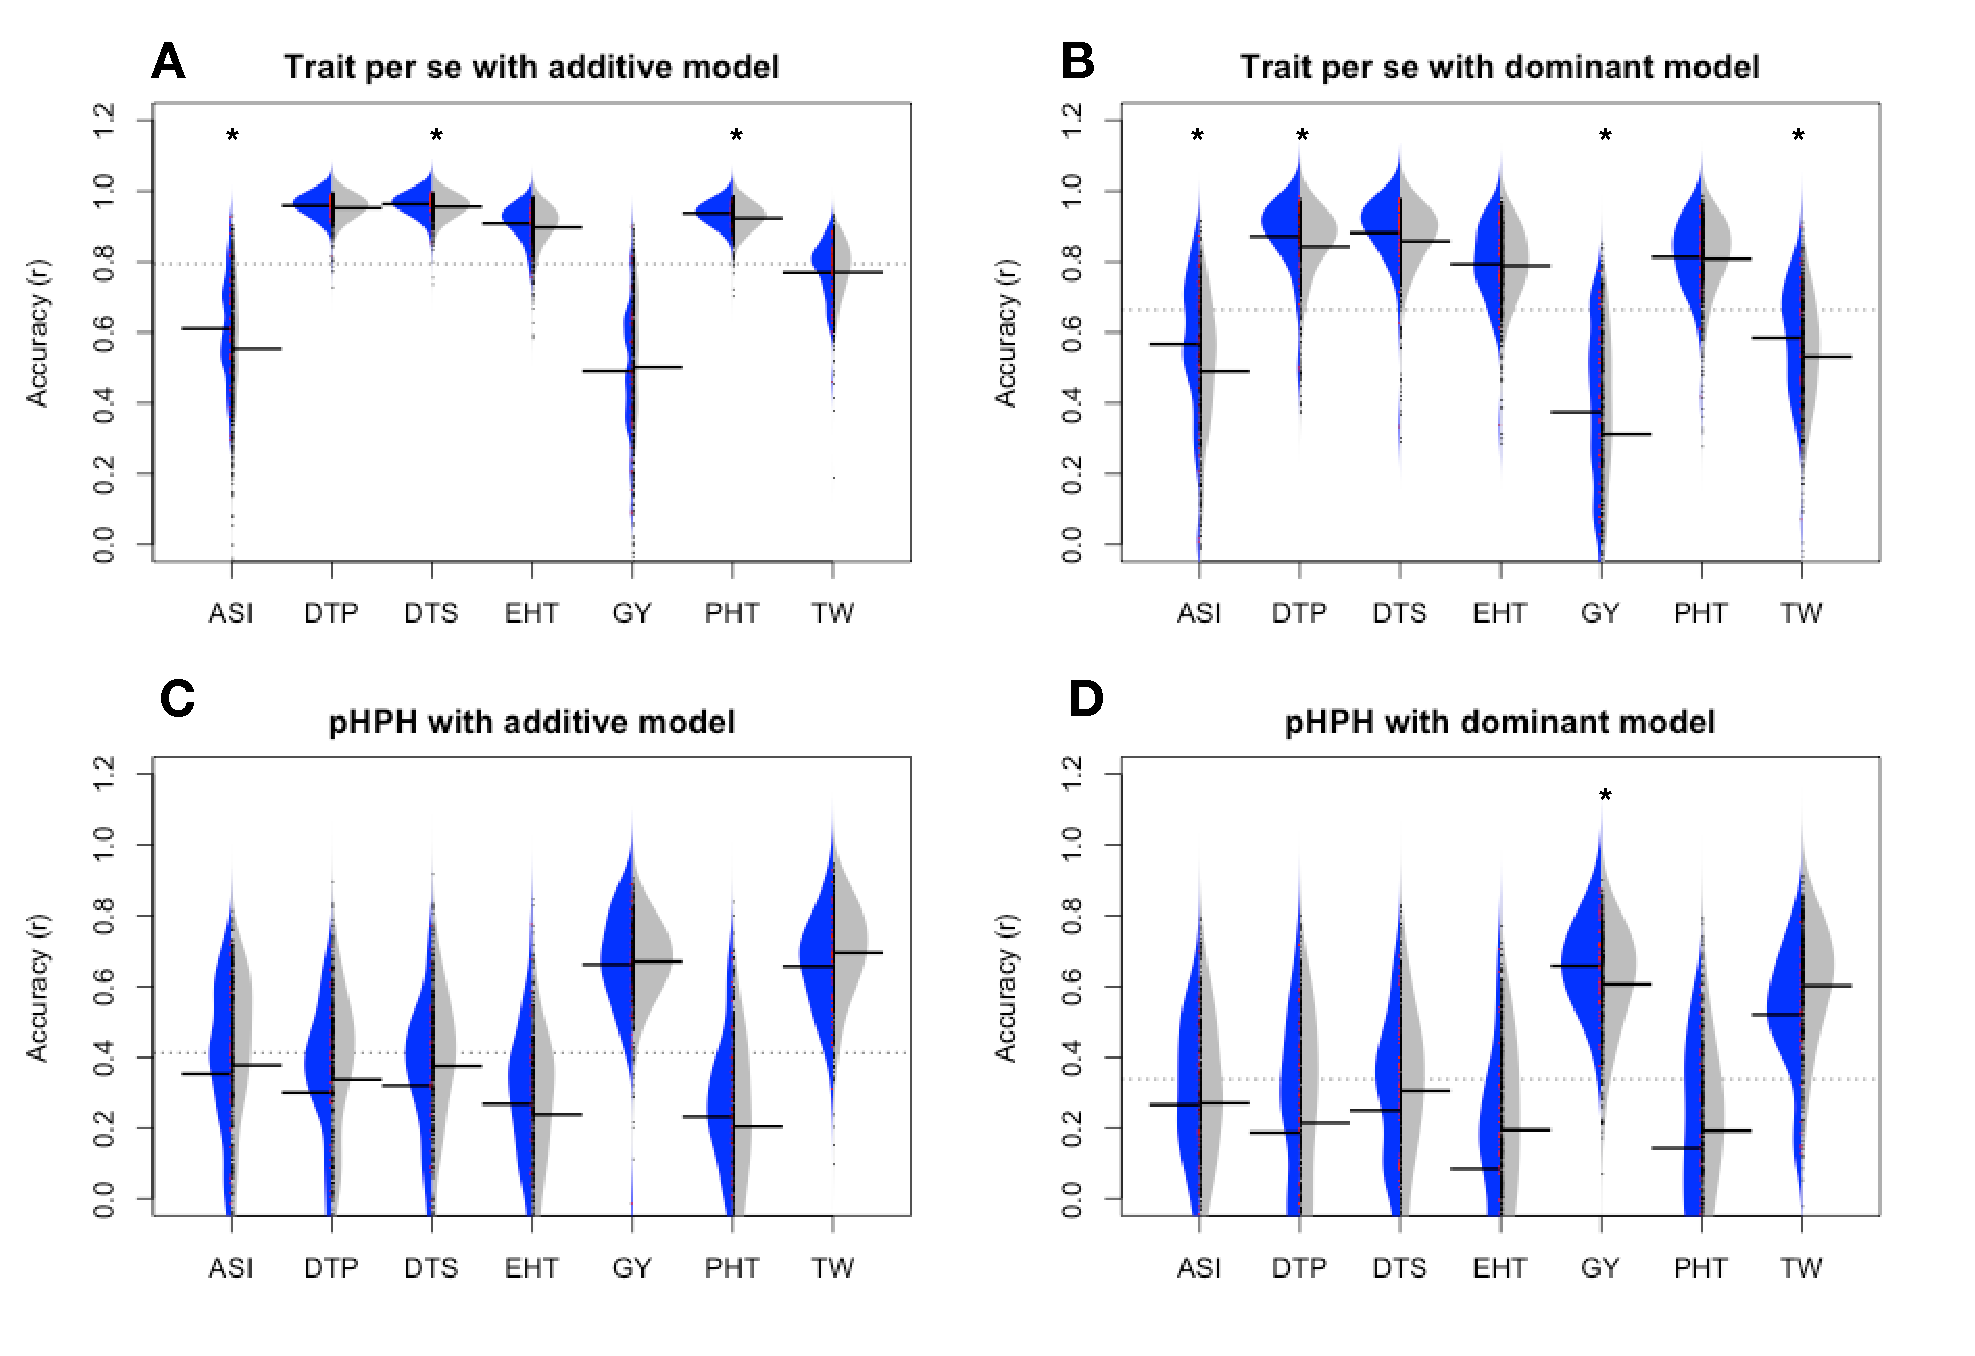
\includegraphics[width=0.8\linewidth]{cvres.pdf}
\captionof{figure}{
\color{black} \textbf{Beanplots of cross-validation accuracies.}
Cross-validation experiments were conducted using genic SNPs and circular shuffled data from the same set of the genic SNPs for traits \emph{per se} (\textbf{A, B}) and pHPH (\textbf{C, D}) under additive (\textbf{A, C}) and dominant (\textbf{B, D}) models. Accuaries from the real data were plotted on the left side of the bean (blue) and permutation results plotted on the right (grey). Horizotal bars on beans indicate mean accuracies. The grey dashed line indicates the overall average accuracy. Stars indicate significantly improved cross-validation accuracies.
}
\end{center}\vspace{1cm}


%----------------------------------------
% SUPPLEMENTARY FIGURES
%----------------------------------------

\pagebreak
\beginsupplement
\section*{SUpporting Information}


%Figure
\begin{center}\vspace{1cm}
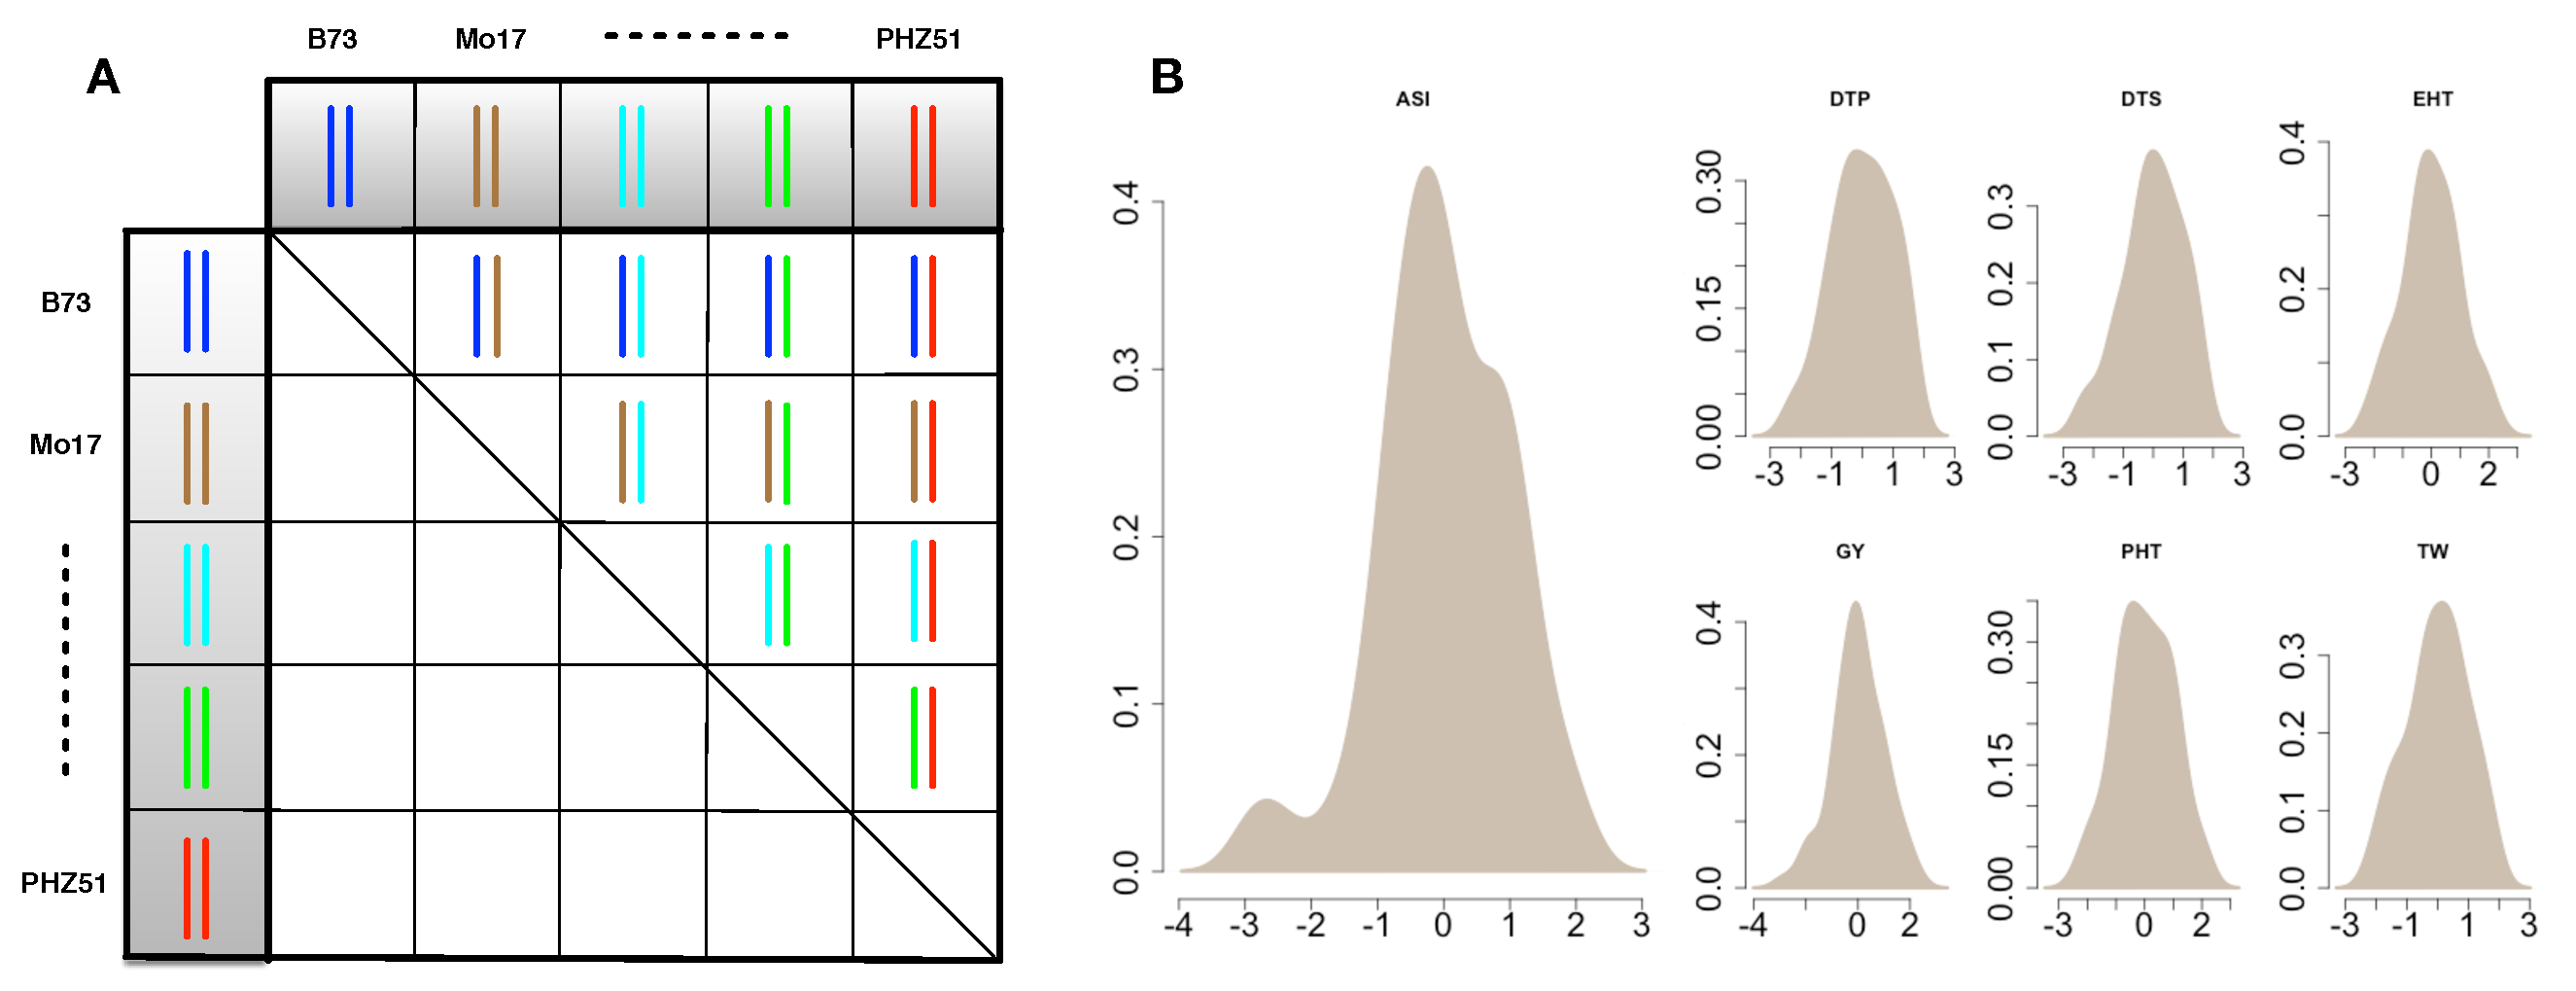
\includegraphics[width=0.8\linewidth]{pvp.pdf}
\captionof{figure}
{\color{black} \textbf{Diallel experimental design and distribution of phenotypic data.}
\textbf{(A)} Twelve maize inbred lines were selected and crossed in a half diallel. Ten of these (LH1, LH123HT, LH82, PH207, 4676A, PHG39, PHG47, PHG84, PHJ40, PHZ51) are proprietary inbreds that have expired from Plant Variety Protection (PVP) and represent the lineage of key heterotic germplasm pools used in present-day commercial corn hybrids. Two of them are important public inbreds, B73 and Mo17. \textbf{(B)} Phenotypic data were collected for anthesis-silking interval (ASI, in days), days to 50\% pollen shed (DTP), days to 50\% silking (DTS), ear height (EHT, in cm), grain yield adjusted to 15.5\% moisture (GY, in bu/A), plant height (PHT, in cm), and test weight (TW, in pounds). Analyses were carried out on the traits per se as well as percent high parent heterosis (pHPH).
}
\end{center}\vspace{1cm}



\begin{center}\vspace{1cm}
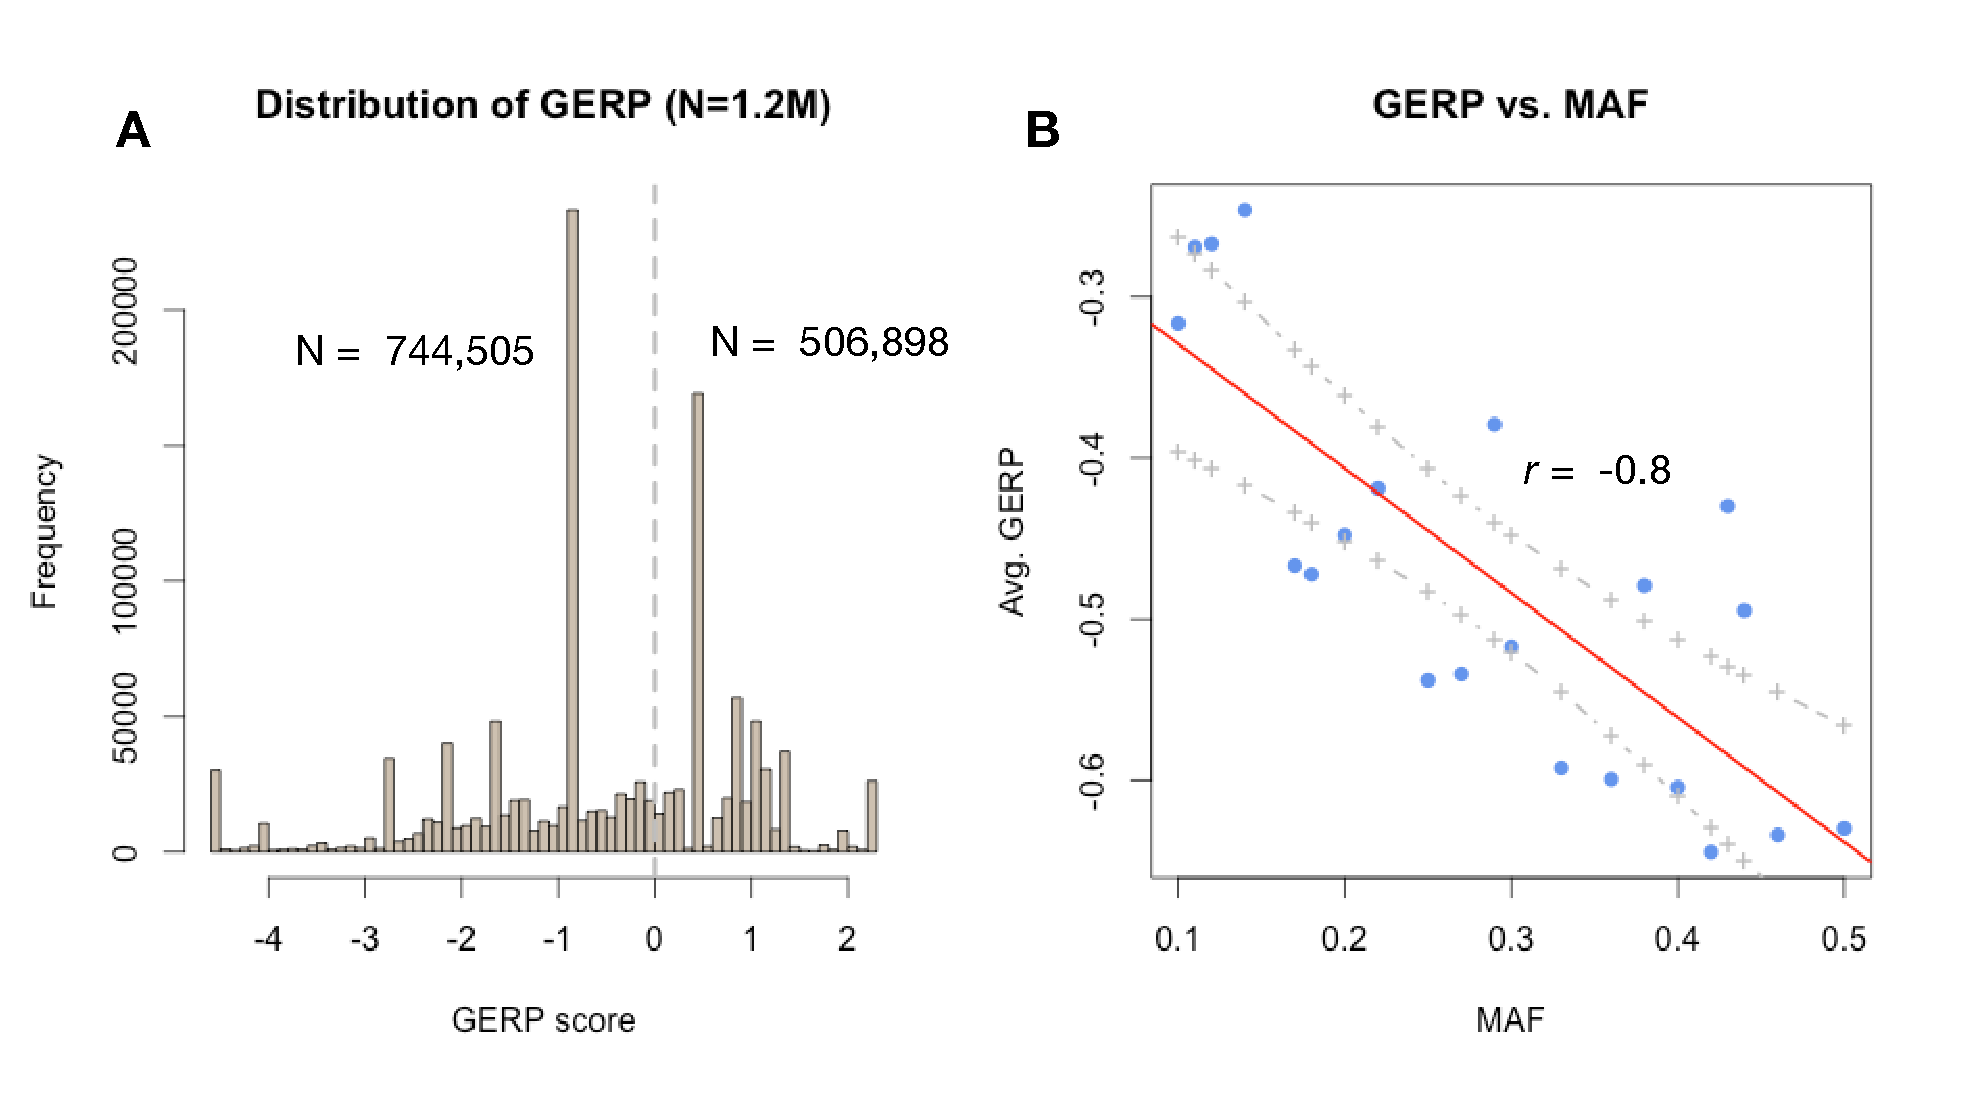
\includegraphics[width=0.8\linewidth]{gerp.pdf}
\captionof{figure}{
\color{black} \textbf{GERP distribution of SNPs and relationship between GERP and minor allele frequency.}
\textbf{(A)} GERP scores were obtained for $\sim$1.2 million ($\sim$10\%) SNPs. Of these, 506,898 (42\%) were under evolutionary constraint and considered as deleterious variants. 
\textbf{(B)} Mean GERP scores were calculated for each bin (bin size = 0.01) of minor allele frequency (MAF). It shows that variants at conserved sites are maintained at low frequency. The red line and grey lines define the regression and its 95\% confidence interval.}
\end{center}\vspace{1cm}





\begin{figure}[here]
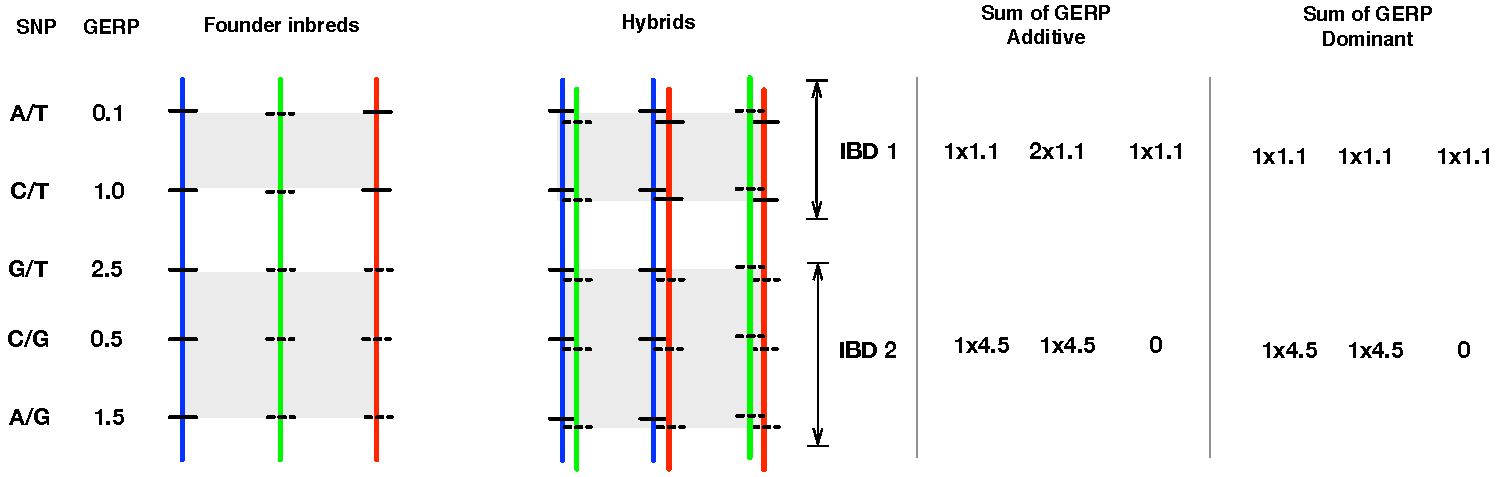
\includegraphics[width=0.9\textwidth]{gerpIBD.pdf}
\caption{
\textbf{Incoporation of conservation information into IBD blocks.}
Regions of the genome that are identical by descent (IBD) among the 12 inbreds were identified using Beagle \citep{Browning2009}.  The GERP scores of SNPs in an IBD block were summed under both additive and dominant models. Under the additive model, 2 x GERP score was assigned to genotypes homozygous for the non-reference allele, 1 x GERP score was assigned to heterozygotes, and 0 was assigned to the homozygous reference genotype. Under the dominant model, 1 x GERP score was assigned to both genotypes with a nonreference allle and 0 to the homozygous reference genotype.}
\label{fig:gerpibd}
\end{figure}




\end{document}
%-----------------------------------------------------------------------------------------------------------------
%-----------------------------------------------------------------------------------------------------------------
% END DOCUMENT
%-----------------------------------------------------------------------------------------------------------------
%-----------------------------------------------------------------------------------------------------------------
% -/\/\/\/\/\/\/\/\/\/\/\/\/\/\/\/\/\/\/\/\/\/\/\/\/\/\/\/\/\/\/\/\/\/\/\/\/\/\/\/\/\/\/\/\/\/\/\/\/\/\/\/\/\/\/\/\/\/\/\/\/\/\/\/\/\/\/\/\/\/\/\/\/\/\/\/\/\/\/\/\/\-
%  -X-X-X-X-X-X-X-X-X-X-X-X-X-X-X-X-X-X-X-X-X-X-X-X-X-X-X-X-X-X-X-X-X-X-X-X-X-X-X-X-X-X-X-X-X-X-
% -\/\/\/\/\/\/\/\/\/\/\/\/\/\/\/\/\/\/\/\/\/\/\/\/\/\/\/\/\/\/\/\/\/\/\/\/\/\/\/\/\/\/\/\/\/\/\/\/\/\/\/\/\/\/\/\/\/\/\/\/\/\/\/\/\/\/\/\/\/\/\/\/\/\/\/\/\/\/\/\/\/-